\documentclass[letterpaper,11pt]{article}
\usepackage[paper=letterpaper,top=2cm,bottom=2cm,left=2.5cm,right=2.5cm]{geometry}
\usepackage[spanish]{babel}
\usepackage[dvips]{epsfig}
\usepackage[utf8]{inputenc}
\usepackage[mathcal]{euscript}
\usepackage{tabularx}

\begin{document}

\title{\textsc{Space Planning Problem 3D}}
\author{\large{Sergio Ahumada Navea} \\ \texttt{san@inf.utfsm.cl}}
\date{29 de julio de 2005}

\maketitle

\begin{abstract}
Dado un conjunto finito de cubos, se trata de
determinar sus posiciones dentro de un ``bin'' o ``contenedor'',
debiendo cumplir ciertas restricciones de conteni\-bi\-li\-dad y superposición.
Estas condiciones dicen relación con el hecho de que todos los objetos
deben quedar dentro del contenedor,
así como ninguno de ellos puede quedar superpuesto con sus adyacentes.
Este problema es $\mathcal{NP}$-duro en el sentido que no es posible
resolverlo usando técnicas completas en tiempos reducidos, ya que a
medida que crece la cantidad de objetos la computación aumenta en orden
exponencial.
Este trabajo presenta un modelo de programación lineal mixta
para representar el problema de \texttt{carga de container} y lo intenta
resolver utilizando la herramienta \textit{Lindo}.
\end{abstract}

\section{Introducción\label{sec:introduccion}}

Los problemas de Carga de Containers (Container Loading Problem) y
los problemas de Empaquetamiento (Bin Packing Problem) son ampliamente
usados en áreas como Diseño de circuitos VLSI, Carga de pallets, Carga
de camiones, etc. \\

En general, los problemas de Space Planning 3D han acaparado la atención
de muchos investigadores en el último tiempo, donde cada uno ha desarrollado
diversas técnicas de resolución que hacen el problema más interesante. Entre
las variantes de este problema están aquellos que sólo utilizan un tipo de cubos;
aquellos denominados ``guillotinables'' o que intentan realizar un orden tal que
es posible cortar de forma perfecta el contenedor con un plano imaginario; aquellos
en que se deben depositar los objetos de arriba hacia abajo, etc. \\

Los problemas de empaquetamiento (Bin Packing Problem) describen la
consistencia de combinaciones de pequeños objetos geométricos en grandes
superficies. En el caso de problemas del tipo Bin Packing las
superficies, $S$, son definidas vacias y se necesita posicionar una
cierta cantidad, $n$, de objetos en su interior. Los objetos no pueden
superponerse ni pueden quedar fuera de la superficie definida, estos
objetos no podrán rotarse, debido a que en el caso 3D la cantidad de
posibles posiciones de un objeto dificulta la resolución del problema.
Además, todos los objetos deben ser puestos en su totalidad en $S$. \\

En este trabajo se presenta el problema combinatorial, en la cual se
trata de ubicar objetos de ciertas dimensiones dadas sobre un volumen
determinado sin que ellos salgan de dicho volumen o se traslapen. \\

La sección~\ref{sec:estado_del_arte} da una mirada general a como es visto
el problema en la actualidad, destacando algunos trabajos sobresalientes.
En la sección~\ref{sec:ejemplo}, se enuncia una instancia sencilla del problema
a modo de ejemplo. En la sección~\ref{sec:alternativas_modelamiento}, se describe en forma
matemática el problema presentado como ejemplo, dando a conocer las
posibles maneras de modelarlo. \\

Se propone en la sección~\ref{sec:modelo_general} un modelo matemático de programación
lineal mixto para su posterior resolución, sin considerar aún la
rotación de los objetos como posible solución.
Utilizando la herramienta \textit{Lingo}, en la sección~\ref{sec:especificacion},
se formula el modelo general de forma de poder resolver automáticamente el
problema. \\

En la sección~\ref{sec:resolucion}, se muestran resultados obtenidos utilizando el
modelo propuesto y la herramienta \textit{Lindo} para resolver el problema.
En la sección~\ref{sec:perspectivas}, se muestran algunos modelos y técnicas
utilizadas para la resolución de este tipo de problemas.
Finalmente, se exponen en la sección~\ref{sec:conclusiones} algunas de las
conclusiones obtenidas de este trabajo.


\section{Estado del Arte\label{sec:estado_del_arte}}

El problema de empaquetamiento o planeación de espacio no sólo esta orientado
a 3 dimensiones, si no que también podemos encontrar problemas de planeamiento
en una y dos dimensiones. Actualmente no existen metodologías de resolución
para este tipo de problemas en un tiempo polinomial, por lo que este tipo
de problemas se clasifican como $\mathcal{NP}$-complejos. \\

Existen, sin embargo, algoritmos como the \textit{First Fit Algorithm}, el cual
posiciona los bloques, u objetos bidimensionales en el orden en que vienen
llegando y busca el primer lograr de calce para cada uno. El problema es que
este algoritmo, difiere del óptimo en aproximadamente un 70\% (Hoffman 1998, p. 171).
Otra estrategia consiste en ordenar primero los objetos desde el más grande
hasta llegar al más pequeño, sin embargo, este método, difiere también del
óptimo, sin embargo, lo hace en aproximadamente un 22\%. \\

Sin embargo, existen modelos más formales para plantear este tipo de problemas,
dadas sus restricciones de espacio y posicionamiento. \\

Por ejemplo, al momento de cortar una plancha de madera para construir una serie
de muebles, es necesario minimizar la cantidad de espacio desperdiciado,
producto de los cortes en la madera, a modo de maximizar la cantidad de
paneles por plancha de madera (Planeación en 2D). \\

Nosotros nos enfocaremos exclusivamente a la planeación en 3 dimensiones, la cual
posee una amplia gama de aplicaciones, como pueden ser el almacenaje de carga en
los aeroplanos, llenado de containeres en forma óptima y, en general, todo lo que
concierne al llenado de espacios tridimensionales en forma óptima. \\

En la actualidad existen software para llevar a cabo diversas tareas de llenado 3D
en forma óptima, como es el caso de 3D Load PackPacker V.1.7x, el cual posee una
base de datos con la información de todos los containeres que utiliza y todos los
tamaños de paquetes para el posible llenado. De esta forma analiza todas las
posibilidades y retorna la que menor espacio perdido tiene. Se ve que este método
de comparaciones es bastante bueno en el caso de formas predefinidas, sin embargo,
esto no es aplicable a casos que no se encuentran en la base de datos del SW en cuestión. \\

Al problema de planeación en 3D se le pueden agregar ciertas modificaciones (Restricciones)
como sería el caso de cargar un container, en el cual existen ciertos paquetes que no
pueden estar con la tapa hacia abajo, otros que tienen que soportar a los que están más
arriba, algunos que no tienen una forma regular, etc. Sin embargo nosotros desarrollaremos
una simplificación de esto, en que todos los paquetes tienen una forma regular y pueden
estar ubicados en cualquier parte del espacio limitado por nuestras restricciones de
posición y ubicación (Traslape).


\section{Ejemplo\label{sec:ejemplo}}
Se propone un ejemplo muy sencillo para ser resuelto posteriormente,
el cual consiste en determinar la mínima altura que debe tener una caja para
empaquetar computadores en su interior. Cada computador tiene tres tipos de piezas:
monitor, cpu y accesorios. \\

Para adecuarnos al problema, se consideró a cada uno de estos tres objetos
con formas rectangulares de dimensiones ($2\times 2\times 2$);
($2\times 1\times 2$) y ($1\times 1\times 1$); de alto, ancho y profundidad
respectivamente. \\

El contenedor consiste en una superficie $S_1$ de dimensiones
$H=4$ y $W=4$ de alto y ancho respectivamente. El cuadro~\ref{tabla:uno}
muestra doce objetos (cuatro computadores, con tres tipos de partes cada
uno) para ser posicionados en la supeficie $S_1$. \\

Para resolver este ejemplo, se considera minimizar la profundidad $D$
del contenedor de manera tal que los doce objetos definidos quepan en $S_1$.

\begin{table}[h]
\begin{center}
\begin{tabular}{||c|c c c||c|c c c||c|c c c||}
\hline\hline
$i$ & $h_i$ & $w_i$ & $d_i$ & $i$ & $h_i$ & $w_i$ & $d_i$ & $i$ & $h_i$ & $w_i$ & $d_i$ \\ \hline
\textbf{1} & 2 & 2 & 2 & \textbf{5} & 2 & 1 & 2 & \textbf{9} & 1 & 1 & 1 \\
\textbf{2} & 2 & 2 & 2 & \textbf{6} & 2 & 1 & 2 & \textbf{10} & 1 & 1 & 1 \\
\textbf{3} & 2 & 2 & 2 & \textbf{7} & 2 & 1 & 2 & \textbf{11} & 1 & 1 & 1 \\
\textbf{4} & 2 & 2 & 2 & \textbf{8} & 2 & 1 & 2 & \textbf{12} & 1 & 1 & 1 \\
\hline\hline
\end{tabular}
\caption{Objetos de instancia sencilla}
\label{tabla:uno}
\end{center}
\end{table}

\pagebreak

\section{Alternativas de modelamiento\label{sec:alternativas_modelamiento}}

Para cumplir con la definición del problema, se propone un modelo de
programación lineal entera mixta, en el cual se desean obtener la terna de
coordenadas inferior-izquierda-trasera (ver figura~\ref{fig:fig_2_1})
de cada uno de los $i$ objetos en sus componentes $X$, $Y$ y $Z$. \\

\begin{figure}[!htb]
 \centering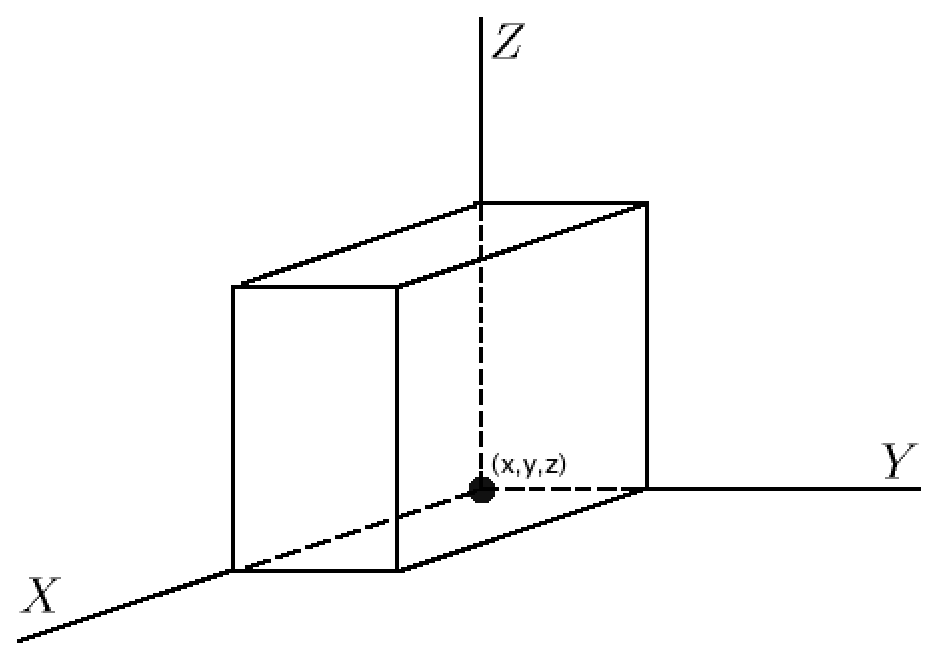
\epsfig{file=fotos/cubo_plano2.eps,width=9cm}
 \caption{Coordenadas $(x,y,z)$ a obtener en la resolución del problema}
 \label{fig:fig_2_1}
\end{figure}

\subsection{Modelamiento}

Un primer acercamiento es considerar la relación que existe entre dos
objetos adyacentes en el espacio, enumerando las posibles combinaciones
de a pares cumpliendo con las restricciones de superposición y contenibilidad
de los objetos dentro de $S_1$. \\

Existen seis restricciones para controlar la superposición de objetos,
estas serán co\-dificadas teniendo en cosideración lo siguiente: \\

\textit{Proposición: Dos objetos $i$ y $j$ no estarán superpuestos si
al menos una de las siguientes restricciones es satisfecha:}
\begin{center}
\begin{tabular}{l p{1cm} c}
Objeto $i$ está a la izquierda de $j$ & & $x_i + w_i \le x_j$ \\
Objeto $i$ está abajo de $j$          & & $y_i + h_i \le y_j$ \\
Objeto $i$ está a la derecha de $j$   & & $x_i - w_j \ge x_j$ \\
Objeto $i$ está arriba de $j$         & & $y_i - h_j \ge y_j$ \\
Objeto $i$ está detrás de $j$         & & $z_i + d_i \le z_j$ \\
Objeto $i$ está delante de $j$        & & $z_i - d_j \ge z_j$ \\
\end{tabular}
\end{center}

Si $H$, $W$ y $D$ son las dimensiones de la superficie $S$, alto, ancho y
profundidad res\-pectivamente, se introducen tres variables binarias
$p_{ij}$, $q_{ij}$ y $r_{ij}$ que permitirán activar solamente una de
las inecuaciones mutamente excluyentes anteriores. \\
\pagebreak

\subsection{Formulación matemática}

Considerando lo anterior, la formulación metamática necesaria para
mantener dos objetos adyacentes sin traslape es la siguiente:

\begin{center}
\begin{tabular}{r c l}
$x_i + w_i$ & $\le$ & $x_j + M \times (p_{ij} + q_{ij} + r_{ij})$ \\
$y_i + h_i$ & $\le$ & $y_j + M \times (1 + p_{ij} + q_{ij} - r_{ij})$ \\
$x_i - w_j$ & $\ge$ & $x_j - M \times (1 + p_{ij} - q_{ij} + r_{ij})$ \\
$y_i - h_j$ & $\ge$ & $y_j - M \times (2 + p_{ij} - q_{ij} - r_{ij})$ \\
$z_i + d_i$ & $\le$ & $z_j + M \times (1 - p_{ij} + q_{ij} + r_{ij})$ \\
$z_i - d_j$ & $\ge$ & $z_j - M \times (2 - p_{ij} + q_{ij} - r_{ij})$ \\
\end{tabular}
\end{center}

Además, es necesario considerar la contenibilidad de los objetos dentro
de la superficie $S_1$, asegurando que no es posible sobrepasar los
límites máximos $H$, $W$ y $D$ de la superficie. \\

\begin{center}
\begin{tabular}{r c l}
$x_i + w_i$ & $\le$ & $W$ \\
$y_i + h_i$ & $\le$ & $H$ \\
$z_i + d_i$ & $\le$ & $D$ \\
\end{tabular}
\end{center}


\section{Modelo general\label{sec:modelo_general}}

\begin{itemize}
\item {\bf Objetivo} \\[6pt]
Ubicar $n=12$ objetos en una superficie cúbica $S$, sin que
ellos se traslapen y quepan en su totalidad, minimizando su
volumen.
\item {\bf Función Objetivo} \\[6pt]
$\min z = D$
\item {\bf Parámetros} \\[6pt]
\begin{tabular}{p{0.5cm} l}
$H$      & Alto fijo de la superficie rectangular $S$ \\
$W$      & Ancho fijo de la superficie rectangular $S$ \\
$n$      & Número de objetos a posicionar en $S$ \\
$h_i$    & Alto del objeto $i$ $(1 \le i \le n)$ \\
$w_i$    & Ancho del objeto $i$ $(1 \le i \le n)$ \\
$d_i$    & Profundidad del objeto $i$ $(1 \le i \le n)$ \\
\end{tabular}
\item {\bf Variables} \\[6pt]
\begin{tabular}{p{0.5cm} l}
$D$      & Profundidad de la superficie rectangular $S$ \\
$x_i$    & Coordenada inferior izquierda trasera en el eje $X$ del objeto $i$ $(1 \le i \le n)$ \\
$y_i$    & Coordenada inferior izquierda trasera en el eje $Y$ del objeto $i$ $(1 \le i \le n)$ \\
$z_i$    & Coordenada inferior izquierda trasera en el eje $Z$ del objeto $i$ $(1 \le i \le n)$ \\
$p_{ij}$ & Variable de codificación del objeto $i$ respecto al objeto $j$ $(1 \le i < j \le n)$ \\
$q_{ij}$ & Variable de codificación del objeto $i$ respecto al objeto $j$ $(1 \le i < j \le n)$ \\
$r_{ij}$ & Variable de codificación del objeto $i$ respecto al objeto $j$ $(1 \le i < j \le n)$ \\
\end{tabular} \\
\pagebreak
\item {\bf Restricciones}
\begin{itemize}
\item[1.] Mantención de los objetos dentro de la superficie $S$: \\[6pt]
\begin{tabular}{p{9.5cm} l}
$x_i + w_i \le W$, & $1 \le i \le n$ \\
$y_i + h_i \le H$, & $1 \le i \le n$ \\
$z_i + d_i \le D$, & $1 \le i \le n$ \\
\end{tabular} \\
\item[2.] Restricciones de superposición de los objetos: \\[6pt]
\begin{tabular}{p{9.5cm} l}
$x_i + w_i \le x_j + M \times (p_{ij} + q_{ij} + r_{ij})$, & $1 \le i < j \le n$ \\
$y_i + h_i \le y_j + M \times (1 + p_{ij} + q_{ij} - r_{ij})$, & $1 \le i < j \le n$ \\
$x_i - w_j \ge x_j - M \times (1 + p_{ij} - q_{ij} + r_{ij})$, & $1 \le i < j \le n$ \\
$y_i - h_j \ge y_j - M \times (2 + p_{ij} - q_{ij} - r_{ij})$, & $1 \le i < j \le n$ \\
$z_i + d_i \le z_j + M \times (1 - p_{ij} + q_{ij} + r_{ij})$, & $1 \le i < j \le n$ \\
$z_i - d_j \ge z_j - M \times (2 - p_{ij} + q_{ij} - r_{ij})$, & $1 \le i < j \le n$ \\
\end{tabular} \\
\item[2.1] Eliminación de casos no posibles: \\[6pt]
\begin{tabular}{p{9.5cm} l}
$p_{ij} + q_{ij} \le 1$ & $1 \le i < j \le n$ \\
$p_{ij} + q_{ij} + r_{ij} \le 2$ & $1 \le i < j \le n$ \\
\end{tabular} \\
\item[3.] No negatividad de las variables enteras: \\[6pt]
\begin{tabular}{p{0.6cm} r p{0.5cm} l}
& $x_i, y_i, z_i \ge 0$, & & $1 \le i \le n$ \\
\end{tabular} \vspace{5pt}
\item[4.] Variables binarias: \\[6pt]
\begin{tabular}{r p{0.5cm} l}
$p_{ij}, q_{ij}, r_{ij} \in \{0,1\}$, & & $1 \le i < j \le n$ \\
\end{tabular} \\
\end{itemize}
\end{itemize}


\pagebreak

\section{Especificación usando Lingo\label{sec:especificacion}}

\scriptsize
\begin{verbatim}
MODEL:
TITLE Bin Packing 3D;

SETS:
 WIDTH  / 1..3 /: X, W;
 HEIGHT / 1..3 /: Y, H;
 DEPTH  / 1..3 /: Z, D;
 LINKS (WIDTH, HEIGHT) | &2 #GT# &1: P, Q, R;
ENDSETS

DATA:
 HT = 4;
 WT = 4;
 MT = 1000;
 W = 2 2 4;
 H = 2 2 2;
 D = 4 4 4;
ENDDATA

! Funcion objetivo;
[FUNC_OBJ] MIN = DT;

! Mantencion objetos dentro de la superficie;
@FOR(WIDTH(I): [DENTRO_X] X(I) + W(I) <= WT);
@FOR(HEIGHT(I):[DENTRO_Y] Y(I) + H(I) <= HT);
@FOR(DEPTH(I): [DENTRO_Z] Z(I) + D(I) <= DT);

! Superposicion de objetos;
@FOR(LINKS(I,J) | I #LT# J: [SUPER1]
    X(I) + W(I) <= X(J) + MT * (P(I,J) + Q(I,J) + R(I,J)));

@FOR(LINKS(I,J) | I #LT# J: [SUPER2]
    X(I) - W(J) >= X(J) - MT * (1 + P(I,J) - Q(I,J) + R(I,J)));

@FOR(LINKS(I,J) | I #LT# J: [SUPER3]
    Y(I) + H(I) <= Y(J) + MT * (1 + P(I,J) + Q(I,J) - R(I,J)));

@FOR(LINKS(I,J) | I #LT# J: [SUPER4]
    Y(I) - H(J) >= Y(J) - MT * (2 + P(I,J) - Q(I,J) - R(I,J)));

@FOR(LINKS(I,J) | I #LT# J: [SUPER5]
    Z(I) + D(I) <= Z(J) + MT * (1 - P(I,J) + Q(I,J) + R(I,J)));

@FOR(LINKS(I,J) | I #LT# J: [SUPER6]
    Z(I) - D(J) >= Z(J) - MT * (2 - P(I,J) + Q(I,J) - R(I,J)));

! Restricciones debiles;
@FOR(LINKS(I,J) | I #LT# J: [DEBIL1]
    P(I,J) + Q(I,J) + R(I,J) <= 2);

@FOR(LINKS(I,J) | I #LT# J: [DEBIL2]
    P(I,J) + Q(I,J) <= 1);

! Variables binarias;
@FOR(LINKS: @BIN(P));
@FOR(LINKS: @BIN(Q));
@FOR(LINKS: @BIN(R));

! Variables no negativas;
@FOR(WIDTH: @GIN(X));
@FOR(HEIGHT:@GIN(Y));
@FOR(DEPTH: @GIN(Z));

END
\end{verbatim}
\normalsize

\pagebreak

\section{Benchmarks\label{sec:benchmark}}

\subsection{Benchmarks del proyecto}

Se realizaron pruebas con distintos tipos de tamaño de problemas. Estos tipos de problemas fueron generados a partir de los casos de pruebas utilizados en~\cite{bib:martello00threedimensional}. \\

Dada una superficie de dimensiones $W$ y $H$, se considerarán cinco tipos de items distintos, a saber:

\begin{itemize}
 \item Tipo 1: $w_j$ u.d. en $[1, \frac{1}{2}W]$, $h_j$ u.d. en $[\frac{2}{3}H, H]$, $d_j$ u.d. en $[\frac{2}{3}D, D]$
 \item Tipo 2: $w_j$ u.d. en $[\frac{2}{3}W, W]$, $h_j$ u.d. en $[1, \frac{1}{2}H]$, $d_j$ u.d. en $[\frac{2}{3}D, D]$
 \item Tipo 3: $w_j$ u.d. en $[\frac{2}{3}W, W]$, $h_j$ u.d. en $[\frac{2}{3}H,H]$, $d_j$ u.d. en $[1, \frac{1}{2}D]$
 \item Tipo 4: $w_j$ u.d. en $[\frac{1}{2}W, W]$, $h_j$ u.d. en $[\frac{1}{2}H,H]$, $d_j$ u.d. en $[\frac{1}{2}D,D]$
 \item Tipo 5: $w_j$ u.d. en $[1,\frac{1}{2}W]$, $h_j$ u.d. en $[1,\frac{1}{2}H]$, $d_j$ u.d. en $[1, \frac{1}{2}D]$
\end{itemize}

Para obtener cinco clases de instancias de prueba se considera que para cada clase $k$ ($k=1,\ldots,5$), cada item es de tipo $k$ con una probabilidad de 60\%, y de los otros cuatro tipos con probabilidad de 10\% cada uno. \\

Un segundo grupo de clases se puede obtener de la generalización de las instancias presentadas por Berkey y Wang. Se definen tres clases como sigue:

\begin{itemize}
 \item Clase 6: $W=H=10$, items con $w_j, h_j, d_j$ u.d. en $[1, 10]$.
 \item Clase 7: $W=H=40$, items con $w_j, h_j, d_j$ u.d. en $[1, 35]$.
 \item Clase 8: $W=H=100$, items con $w_j, h_j, d_j$ u.d. en $[1, 100]$.
\end{itemize}

Utilizando estos tipos de items, se procedieron a hacer benchmarks comparando los algoritmos de Branch-and-Bound, provisto por la herramienta ``lp\_solve'' y Enumeración Implicita, programado en C. \\

\begin{table}[!htp]
\centering
\begin{tabular}{||c|l|l|c||}
\hline\hline
Items & B\&B & Enum & Óptimo\\ \hline
3 & 0.007s & 0.003s & Y \\
4 & 0.010s & 0.006s & Y \\
5 & 0.065s & 0.007s & Y \\
6 & 0.594s & 0.011s & Y \\
7 & 1.414s & 0.024s & Y \\
10 & -- & 12.786s & Y \\
14 & -- & 22.010s & Y \\
16 & -- & 35.463s & Y \\ \hline\hline
\end{tabular}
\caption{Benchmarks Branch-and-Bound v/s Enumeración implicita}\label{tabla:07_01}
\end{table}
\pagebreak

\subsection{Benchmarks clásicos}

En la sección describiremos un algoritmo enumerativo para la solución exacta de 3D-SP. Este algoritmo resuelve sub-problema
s asociados repetidamente, en que todos los componentes dados de un subgrupo \(\bar{J}\) tienen que ser situados en un solo
 compartimiento, si es posible. Este problema es NP-duro en el buen sentido, desde la resolución de casos especiales en que
 todos los componentes tienen la misma profundidad $d_j=D$ y el mismo alto $h_j=H$ resolvemos la pregunta si una instancia
del problema Space Planning 2D admite una solución sin necesitar mas que H tableros. En la presente sección describiremos u
n algoritmo \emph{Branco-and-bound} para la solución exacta de una versión optimizada del problema (maximizar el volumen to
tal de los ítems empaquetados), que también es usado en uno de los algoritmos que se describen mas adelante.

El problema que consideraremos es seleccionar un subgrupo \(\bar{J}'\le\bar{J}\) de ítems y asignarles coordenadas \((x_j,
y_j, z_j)\) a cada ítem \(j E \bar{J}\) para que ningún ítem quede afuera del tablero o paquete, no queden traslapados y el
 volumen total de los ítems \(\bar{J}'\) sea un máximo. Para el caso de 2 dimensiones se considera una versión del problema
 de la mochila. Presentaremos una generalización no trivial del caso de 2 dimensiones y daremos un algoritmo efectivo para
este problema. Asumiremos que el origen del sistema de coordenadas esta en la esquina inferior izquierda del tablero.\\
En cada nodo de las ramas del árbol de decisión, que describiremos posteriormente con mayor detalle, una solución parcial q
ue empaqueta los ítems de un subgrupo \(I c \bar{J}\), es incrementado seleccionando y rotando cada ítem \(j E \bar{J}/I\)
y generando nodos descendientes al ubicar j en todos los posibles puntos. Poner un ítem en un punto p significa que su esqu
ina inferior izquierda es posicionada en p.\\

De este modo las coordenadas de p quedan representadas por \((x_j, y_j, z_j)\) : Obviamente el ítem j no puede ser posicion
ado en p si
\(x_p + w_j > W\) o \(y_p + h_j >H\) o \( z_p+d_j >D\). Los puntos que pueden ser considerados se ven reducidos por las sig
uientes propiedades.\\

\emph{Propiedad 1} Cualquier ordenamiento de un tablero puede ser reemplazado por uno equivalente, en que ningún ítem sea m
ovido hacia la izquierda, abajo o atrás.\\
\emph{Propiedad 2} Un Orden óptimo de los ítems existe si \(i < j\), \(X_i + w_i \le x_j\) o \(y_i + h_i \le y_i\) o \(z_i
+ d_i \le z_j\)

\emph{Buscando una posible ubicación para posicionar un ítem} \\

Solucionaremos este problema mediante repeticiones de problemas de 2 dimensiones, considerando las caras x-y como un subcon
junto de los ítems. Así empezaremos con la descripción del algoritmo de dos dimensiones.\\
Dado un ítem I, es fácil encontrar, en dos dimensiones el sistema \emph{C(I)} de puntos de las esquinas que recubre el objeto, asociada a la región factible \emph{S(I)} definida por las caras \emph{x-y} de los ítems en I. Ordenemos los ítems de acuerdo a sus puntos finales \((x_j+w_j,y_j+h_j)\), de modo que los valores \(y_j+h_j\) no se incrementen, rompiendo vínculos con los valores mas grandes de \(x_j+w_j\). El siguiente algoritmo para determinar los puntos de la esquina, consta de tres fases: Primero, ítems extremos son encontrados, i.e., ítems cuyos puntos finales coinciden con un punto en que el entorno cambia de horizontal a vertical. En la segunda fase, puntos de la esquina son definidos como intersecciones entre las líneas que conducen desde puntos finales de ítems extremos. Finalmente esquinas no factibles donde ningún otro ítem \(\bar{J}/I\) pueda entrar, son removidas. Así tenemos el siguiente algoritmo:\\

\begin{figure}[!htb]
\centering
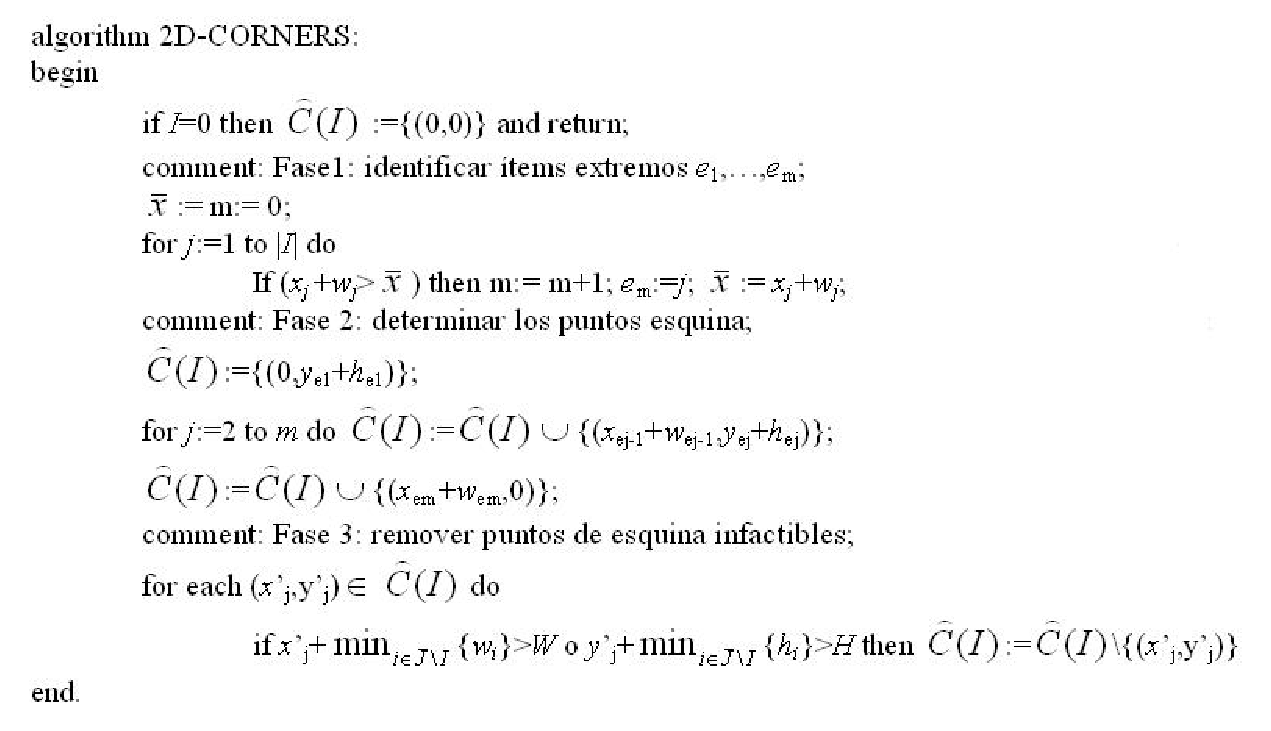
\includegraphics[scale=0.6]{fotos/foto1.eps}
\caption{Algoritmo 2D-CORNERS}
\end{figure}

\begin{figure}[!htb]
\centering
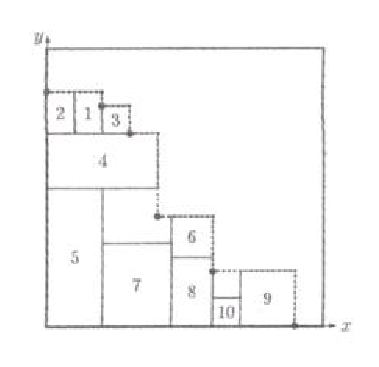
\includegraphics[scale=0.6]{fotos/foto2.eps}
\caption{Envoltura plana del bin}
\end{figure}

Considerando el ejemplo de la figura 2: los ítems extremos 1, 3, 4, 6 y 9 y los puntos de las esquinas resultantes están in
dicados por puntos negros; Fase 3 puede remover algunos de los primeros y/o últimos puntos de las esquinas.\\
La complejidad del 2D-CORNERS es \(O(|I|)\), mas \(O(|I| log |I|)\) para el ordenamiento del ítem inicial, i.e., \(O(n)\) m
as \(O(n log n)\).\\
Asumimos que los puntos de las esquinas resultantes son \(C(I)={(x'_j,y'_j),\dots{},(x'_l,y'_l)}\ne 0\). Entonces el área o
cupada es:

\begin{figure}[!htb]
\centering
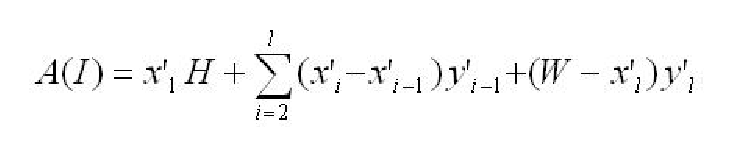
\includegraphics[scale=0.6]{fotos/foto3.eps}
\caption{Área utilizada dentro de la superficie}
\end{figure}

Donde el primero termino es no cero siempre que el punto de la esquina encontrado en la fase 2 sea removido en la fase 3. E
n el caso especial donde \(C(I)=0\), obviamente asignamos \(A(I)=WH\).\\
El algoritmo 2D-CORNERS puede ser usado para determinar el sistema \(C(I)\) de puntos de las esquinas en tres dimensione
s, donde I es el sistema de tres dimensiones actualmente empaquetado dentro del contenedor. Se puede aplicar para z=0 y par
a cada z distinto donde un ítem I termina, mediante incremento de valores. Para tales coordenadas z', 2D-CORNERS puede ser
aplicado a cada subsistema de ítems \(i E I\) que terminan despues de z', es decir:\\

\begin{center}
\(z_i + d_i >z'\)
\end{center}
agregando los puntos de las esquinas resultantes a \(C(I)\). Mediante este camino, uno puede sin embargo obtener algún punt
o falso, desde que son puntos del caso de 2 dimensiones pero no en el caso de 3 dimensiones. Esos puntos son fácilmente rem
ovidos por dominación, donde decimos que el punto \((x'_a,y'_a,z'_a)\) domina a otro punto \((x'_b,y'_b,z'_b)\) que esta es
condido detrás de el. Formalmente esto se escribe así:

\begin{center}
\(x'_a=x'b\) y \( z'_a=y'b\) y \(z'_a < z'_b\)\\
\end{center}
Donde tenemos igualdades en las dos primeras expresiones, asegurando que todos los ítem en frente de \(z'_k\) sean elegidos
 y ahi no se generaran puntos dentro del área. Esto se hace en el siguiente algoritmo, donde la generación de puntos finale
s tan pronto como la coordenada z es encontrada tales ítems no factibles pueden ser posicionados después de el.\\

\begin{figure}[!htb]
\centering
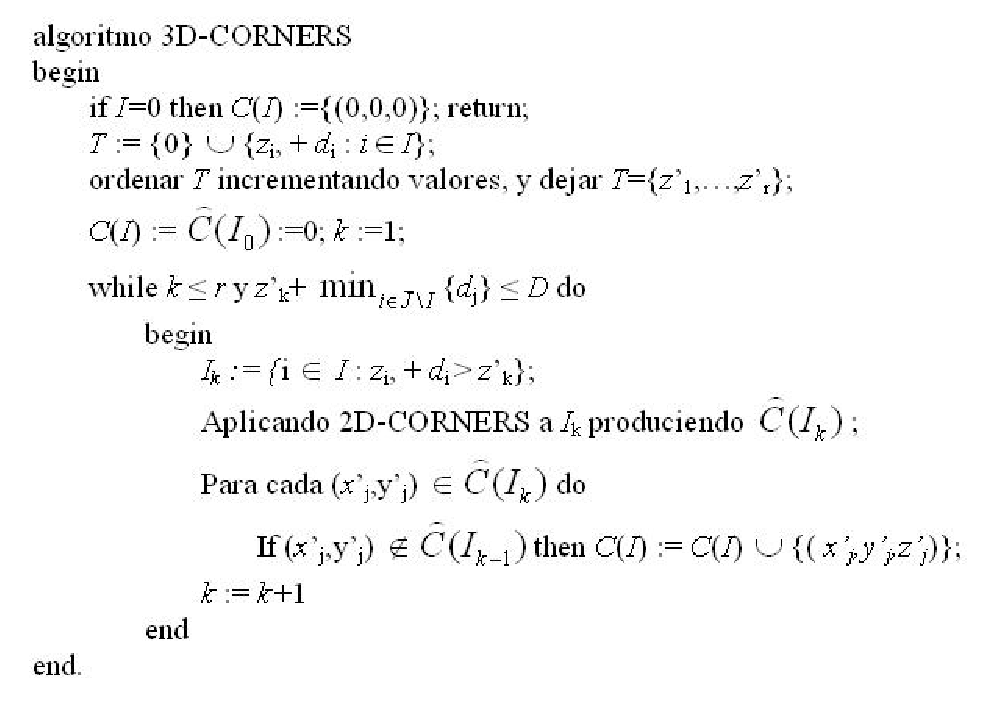
\includegraphics[scale=0.6]{fotos/foto4.eps}
\caption{Algoritmo 3D-CORNERS}
\end{figure}

La complejidad de 3D-CORNERS es \(O(n^2)\) de hecho hay mas coordenadas \(|I|+1\) distintas de  z en  T, y cada sistema \(C(I_k)\) es derivado de 2D-CORNERS en \(O(|I_k|)\), desde que el ordenamiento de ítems puede ser hecho desde el comienzo para los algoritmos. Para cada valor de  \(z'_k\) el chequeo de los puntos requiere \(O(|C(I_k)|)\) en total, desde que ambos \(C(I_k)\) y \(C(I_k)\) son ordenados por incremento de \(x'_j\) y decreciendo \(y'_j\). La complejidad total seguida de la observación de ambas \(|I|\) y \(C(I_k)\) es \(O(n)\).\\

sumiendo que k* es el induce de los I* 3D-CORNERS generados, el volumen V(I) ocupado por los ítems asociado a I es:\\

\begin{figure}[!htb]
\centering
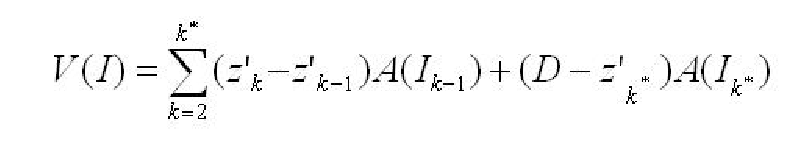
\includegraphics[scale=0.6]{fotos/foto5.eps}
\caption{Volumen utilizado dentro del bin}
\end{figure}

\begin{figure}[!htb]
\centering
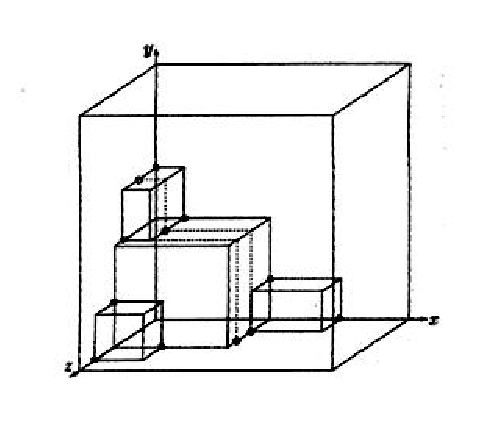
\includegraphics[scale=0.6]{fotos/foto6.eps}
\caption{Envoltura en el espacio 3D}
\end{figure}

\emph{Algoritmos exactos y aproximaciones para 3D-SP.}\\

El algoritmo exacto para 3D-SP esta basado en una descomposición de 2 niveles. Un árbol de ramificaron principal asigna íte
ms a contenedores sin especificar su posición actual, mientras que una versión especializada del algoritmo es usada para lo
s nodos seguros, testeando los sub ítems que pueden ser introducidos dentro de un contenedor simple. Para construir una bue
na solución inicial 2 heurísticas se han definido, una basada en \emph{first-fit-decreasing} y otra basada en la versión \emph{m-cut} del algoritmo ONEBIN\\

\emph{Árbol principal de ramificación}\\

El árbol principal de ramificaciones asigna ítems a los diferentes contenedores especificando su actual posición. Los ítems
 son previamente ordenados de acuerdo a volúmenes decrecientes y la exploración sigue una estrategia de \emph{profundidad-p
rimero}. Sea Z el valor de la solución segura y \(M = {1,\dots{},m}\) el actual sistema de contenedores. Un contenedor de M
 es llamado abierto de otro modo estaría cerrado.\\
En cada nodo de decisión el próximo ítem libre es asignado a todos los contenedores abiertos si \(|M| < Z - 1\) el ítem es
también asignado a un nuevo contenedor.\\
Cuando un ítem k es asignado a un contenedor i que ya contiene un subconjunto, por ejemplo \(\bar{J} \cup k'\). Si el limit
e inferior es mayor que uno para cada k', el contenedor esta cerrado, por lo tanto no se pueden introducir mas ítems en el.
 De otro modo la siguiente regla es testeada. Sea K un subconjunto de los ítems libres que se han generado sobre el limite
inferior. Si una heurística puede encontrar un contenedor para la instancia definida por los ítems en  sabemos que no hay u
na mejor posición posible.\\

\emph{Algoritmos de aproximación}\\

Para obtener una buena cota superior para el nodo raíz del árbol de ramificación y acotar el número de ejecuciones de ONEBIN
, dos diferentes heurísticas son definidas. Dos aproximaciones proveen un complemento computacional. Para desempeños muy ba
jos de una, la otra proporciona desempeños mas elevados, sin embargo la segunda entrega mejores resultados.\\


\pagebreak

\section{Resolución\label{sec:resolucion}}
Se analizó un caso de prueba muy sencillo debido a la cantidad de restricciones
que se deben escribir a medida que aumentan la cantidad de objetos. Se dispondrá
de tres objetos, dos de ellos de dimensiones $(2, 2, 4)$ y uno de dimensiones $(4, 2, 4)$.\\

El caso de prueba consiste en una superficie $S_1$ de dimensiones
$H=4$, $W=4$ y $D=4$ de alto , ancho y profundidad respectivamente. El
cuadro~\ref{tabla:dos} muestra $3$ objetos que sabe caben en la
supeficie $S_1$. Para resolverlo, sólo se considero minimizar la profundidad
del contenedor; el valor de $M$ se fijó en 1000.

\begin{table}[h]
\begin{center}
\begin{tabular}{||c|c c c||}
\hline\hline
$i$ & $w_i$ & $h_i$ & $d_i$ \\ \hline
1 & 2 & 2 & 4 \\
2 & 2 & 2 & 4 \\
3 & 4 & 2 & 4 \\ \hline\hline
\end{tabular}
\caption{Objetos para analizar el primer caso de prueba}
\label{tabla:dos}
\end{center}
\end{table}

Con estos datos se obtuvo el siguiente modelo de programación lineal, como muestra
el cuadro~\ref{tab:table_1}:\\

\begin{table}[!htb]
\scriptsize
\begin{verbatim}
MIN DT

ST
  ! Mantencion objetos dentro de la superficie
   X_1 <= 2
   X_2 <= 2
   X_3 <= 0
   Y_1 <= 2
   Y_2 <= 2
   Y_3 <= 2
   - DT + Z_1 <= - 4
   - DT + Z_2 <= - 4
   - DT + Z_3 <= - 4
  ! Superposicion de objetos
   - 1000 * P_1_2 - 1000 * Q_1_2 - 1000 * R_1_2 + X_1 - X_2 <= - 2
   - 1000 * P_1_3 - 1000 * Q_1_3 - 1000 * R_1_3 + X_1 - X_3 <= - 2
   - 1000 * P_2_3 - 1000 * Q_2_3 - 1000 * R_2_3 + X_2 - X_3 <= - 2
     1000 * P_1_2 - 1000 * Q_1_2 + 1000 * R_1_2 + X_1 - X_2 >= - 998
     1000 * P_1_3 - 1000 * Q_1_3 + 1000 * R_1_3 + X_1 - X_3 >= - 996
     1000 * P_2_3 - 1000 * Q_2_3 + 1000 * R_2_3 + X_2 - X_3 >= - 996
   - 1000 * P_1_2 - 1000 * Q_1_2 + 1000 * R_1_2 + Y_1 - Y_2 <=   998
   - 1000 * P_1_3 - 1000 * Q_1_3 + 1000 * R_1_3 + Y_1 - Y_3 <=   998
   - 1000 * P_2_3 - 1000 * Q_2_3 + 1000 * R_2_3 + Y_2 - Y_3 <=   998
     1000 * P_1_2 - 1000 * Q_1_2 - 1000 * R_1_2 + Y_1 - Y_2 >= - 1998
     1000 * P_1_3 - 1000 * Q_1_3 - 1000 * R_1_3 + Y_1 - Y_3 >= - 1998
     1000 * P_2_3 - 1000 * Q_2_3 - 1000 * R_2_3 + Y_2 - Y_3 >= - 1998
     1000 * P_1_2 - 1000 * Q_1_2 - 1000 * R_1_2 + Z_1 - Z_2 <=   996
     1000 * P_1_3 - 1000 * Q_1_3 - 1000 * R_1_3 + Z_1 - Z_3 <=   996
     1000 * P_2_3 - 1000 * Q_2_3 - 1000 * R_2_3 + Z_2 - Z_3 <=   996
   - 1000 * P_1_2 + 1000 * Q_1_2 - 1000 * R_1_2 + Z_1 - Z_2 >= - 1996
   - 1000 * P_1_3 + 1000 * Q_1_3 - 1000 * R_1_3 + Z_1 - Z_3 >= - 1996
   - 1000 * P_2_3 + 1000 * Q_2_3 - 1000 * R_2_3 + Z_2 - Z_3 >= - 1996
   ! Restricciones debiles
   P_1_2 + Q_1_2 + R_1_2 <= 2
   P_1_3 + Q_1_3 + R_1_3 <= 2
   P_2_3 + Q_2_3 + R_2_3 <= 2
   P_1_2 + Q_1_2 <= 1
   P_1_3 + Q_1_3 <= 1
   P_2_3 + Q_2_3 <= 1
END
\end{verbatim}
\end{table}
\pagebreak

\begin{table}[!htb]
\scriptsize
\begin{verbatim}
   !Variables binarias
   INT P_1_2
   INT P_1_3
   INT P_2_3
   INT Q_1_3
   INT Q_1_2
   INT Q_2_3
   INT R_1_2
   INT R_1_3
   INT R_2_3
   ! Variables no negativas
   GIN X_1
   GIN X_2
   GIN X_3
   GIN Y_1
   GIN Y_2
   GIN Y_3
   GIN Z_1
   GIN Z_2
   GIN Z_3
\end{verbatim}
\caption{Modelo de programación lineal mixto: Formato Lindo}
\label{tab:table_1}
\end{table}

Luego se procedió a correr el programa llegando al resultado
que muestra a continua\-ción el cuadro~\ref{tab:table_3}: \\

\begin{table}[!htb]
\scriptsize
\begin{verbatim}
 OBJECTIVE FUNCTION VALUE

 1)                 4.000000000

 VARIABLES                      VALUE             REDUCED COST
 DT                       4.000000000              0.000000000
 X_1                      0.000000000              0.000000000
 X_2                      2.000000000              0.000000000
 X_3                      0.000000000              0.000000000
 Y_1                      0.000000000              0.000000000
 Y_2                      0.000000000              0.000000000
 Y_3                      2.000000000              0.000000000
 Z_1                      0.000000000              0.000000000
 Z_2                      0.000000000              0.000000000
 Z_3                      0.000000000              0.000000000
 P_1_2                    0.000000000              0.000000000
 Q_1_2                    0.000000000              0.000000000
 R_1_2                    0.000000000              0.000000000
 P_1_3                    0.000000000              0.000000000
 Q_1_3                    0.000000000              0.000000000
 R_1_3                    1.000000000              0.000000000
 P_2_3                    0.000000000              0.000000000
 Q_2_3                    0.000000000              0.000000000
 R_2_3                    1.000000000              0.000000000
\end{verbatim}
\caption{Resultado del modelo de programación lineal mixto}
\label{tab:table_3}
\end{table}
\normalsize

Se puede notar que el total de los objetos fue posicionado correctamente.
Se realizaron pruebas utilizando distintos casos de prueba y distintos métodos
de resolución, los cuales validarian el modelo para el caso específico que
estamos analizando. \\

La interpretación de los datos resultado nos indica que la profundidad óptima
del contenedor es de 4 unidades; las coordenas del objeto 1 son $(0, 0, 0)$ y
las del objeto 2 son $(0, 2, 0)$ considerando la notación $(x, y, z)$. Además,
la variable $p_{12}$ queda activa, por lo cual se cumple sólo una restricción
de superposición indicando que el objeto 1 esta arriba del objeto 2.

\pagebreak

\section{Perspectivas de investigación\label{sec:perspectivas}}

Para la resolución de este tipo de problemas de optimización, se puede seguir la siguiente
metodología, la cual se esta utilizando en la actualidad por diversos software de
estas características:

\begin{itemize}
\item Presentar los datos del problema en una estructura de datos, para poder manejar
      todas las variables de una manera más simplificada y ordenada.
\item Describir cómo sería la inserción de un cubo dentro del contenedor.
\item Presentar un algoritmo de barrido de un solo paso que muestre todos los candidatos
      a ser insertados, con su correspondiente espacio perdido y su complejidad asociada.
\item Cómo representar los datos obtenidos en una estructura de datos.
\end{itemize}

\begin{enumerate}
\item Se utiliza una forma estándar para conectar el caso de 2 dimensiones con el caso
      de 3 dimensiones, en que el primero será la cara frontal del objeto tridimensional.
      En el frente podemos distinguir vértices, bordes y celdas, de este modo, en cada
      celda, se guarda la profundidad de ella. Esta información se guarda en listas doblemente
      enlazadas separadamente. De esta manera se puede representar el interior de un container
      o de un espacio confinado por medio de una estructura de datos.
\item Al insertar un nuevo objeto (caja), la estructura de datos debe ser modificada, para
      que represente la nueva realidad del frente del contenedor. Esto puede resumirse como
      la inserción de un rectángulo, si lo pensamos como un área bidimensional.
\item En el planteamiento de estos algoritmos podemos distinguir dos tipos fundamentales: \\
Heurísticas:
\begin{itemize}
 \item Constructiva.
 \item Búsqueda local por entornos.
 \item Cadenas de movimiento.
\end{itemize}
Metaheurísticas:
\begin{itemize}
 \item Basado en Búsqueda por entornos: Búsqueda tabú; Búsqueda en entorno variable, VNS; GRASP.
 \item Evolutivos basados en población: Algoritmos genéticos; Algoritmos meméticos; Scatter Search.
\end{itemize}
\item Finalmente, los datos obtenidos deben ser representados en una estructura de datos de
      la misma forma en que fueron definidos inicialmente, a modo de mantener una coherencia
      entre la información inicial y la información final, ya que generalmente esto puede
      verse como una capa dentro de algún software especifico de optimización.
\end{enumerate}


\section{Conclusiones\label{sec:conclusiones}}
El problema de planificación de espacio considerado en este trabajo
tiene variadas aplicaciones en la industria. Al ser un problema
$\mathcal{NP}$-duro es muy dificil resolverlo en tiempos acotados a
medida que la cantidad de objetos aumenta. \\

Es por esto que el modelo utilizado es de gran importancia, debido
a que una buena definición de las variables puede incidir de manera
importante en el espacio de búsqueda, el cual es fundamental a la
hora de resolver problemas de este tipo. \\

Las técnicas de resolución también cumplen un papel fundamental cuando
se desea reducir los tiempos de cómputo o se intenta restringir aun más
el problema tratado. Para esto se tienen a disposición las técnicas
completas o incompletas de forma de poder aproximar de buena manera y
obtener un resultado razonable. \\

Las técnicas de enumeración permiten teóricamente
encontrar un óptimo, pero éstas son impracticables cuando superamos un
cierto número de elementos en el dominio de solución. \\

Hemos analizado un caso particular, en el cual el modelo y la herramienta
\textit{Lindo} nos han ayudado a encontrar un valor óptimo para los ejemplos
estudiados y una cota aproximada para el número máximo de objetos que pueden
ser resueltos con ella.


\nocite{*}
\bibliography{referencias}
\bibliographystyle{plain}

\end{document}
